\documentclass[conference]{IEEEtran}
\IEEEoverridecommandlockouts

% Packages
\usepackage{cite}
\usepackage{amsmath,amssymb,amsfonts}
\usepackage{algorithmic}
\usepackage{graphicx}
\usepackage{textcomp}
\usepackage{xcolor}
\usepackage{booktabs}
\usepackage{multirow}
\usepackage{array}

\def\BibTeX{{\rm B\kern-.05em{\sc i\kern-.025em b}\kern-.08em
    T\kern-.1667em\lower.7ex\hbox{E}\kern-.125emX}}

\begin{document}

\title{Efficient Panoramic Semantic Segmentation with Memory Optimization and Boundary-Aware Inference}

\author{\IEEEauthorblockN{Anonymous Authors}
\IEEEauthorblockA{\textit{Institution Name} \\
City, Country \\
email@example.com}
}

\maketitle

% Abstract
\begin{abstract}
Unsupervised domain adaptation for panoramic semantic segmentation requires transferring from labeled perspective source domains to unlabeled panoramic target domains, facing challenges including projection distortion, cross-field-of-view dependencies, and pseudo-label noise. OmniSAM employs a SAM2-style memory mechanism to model panoramic view sequences, but interactions with numerous historical memory tokens significantly increase training costs. This paper proposes a memory-efficient training scheme consisting of Memory Token Compression (MTC) and Sparse Memory Retrieval (SMR): MTC aggregates spatially adjacent redundant memories, while SMR sparsely selects historical tokens by importance, thereby reducing the representation scale entering memory attention; pseudo-label quality optimization serves only as auxiliary exploration. In Cityscapes $\rightarrow$ DensePASS experiments with sam2\_s on 13 classes using a single seed, training time decreases by approximately 22.4\%, with mIoU changing from 60.26 to 60.16 and BFScore from 39.97 to 39.86. Ablation results further demonstrate that token budget reduction is directly correlated with attention overhead reduction, though stronger compression may affect boundaries and small objects. Qualitative comparisons show that both configurations maintain similar major scene structures, with local differences consistent with slight boundary metric degradation. These results support trading moderate accuracy for training efficiency, though cross-dataset and multi-seed stability remain to be verified.
\end{abstract}

\noindent\textbf{Keywords:} Panoramic semantic segmentation; Unsupervised domain adaptation; OmniSAM; Memory mechanism; Token compression; Efficient training


% Main Content
\section{Introduction}
\label{sec:introduction}

Panoramic semantic segmentation predicts semantic categories for each pixel in $360^\circ$ scenes, providing complete surrounding environment representation for autonomous driving and robotics~\cite{yang2021omnirange,ma2021densepass}. Compared to conventional perspective images, equirectangular projection (ERP) covers a larger field of view but introduces significant geometric distortion, regional scale variations, and boundary continuity issues at the horizontal seam. The same road, building, or vehicle may span multiple local views, requiring models to not only recognize local details but also maintain semantic and boundary consistency over long-range contexts. In the Cityscapes~\cite{cordts2016cityscapes} $\rightarrow$ DensePASS~\cite{ma2021densepass} unsupervised domain adaptation (UDA) setting, the source domain provides pixel-level annotations while the target domain contains only unlabeled panoramic images; combined differences in imaging modality, projection structure, and scene distribution make direct transfer of source domain models considerably more difficult. Especially near horizontal seams, distant regions, and elongated structures, local predictions are affected by both projection distortion and the lack of stable scale priors relied upon by perspective models.

When target domain human annotations are unavailable, semantic segmentation typically relies on self-training and pseudo-label construction for supervision. However, distorted regions, view junctions, rare classes, and small objects in panoramic images are more prone to low-confidence or erroneous predictions, and incorrect supervision may accumulate during iterative training. Simply raising pseudo-label thresholds reduces effective pixels and biases toward easily classified categories, while independent prediction over local windows fails to exploit cross-field-of-view structures. Therefore, panoramic UDA~\cite{zhang2022bending,zheng2023dppass,zheng2023datr,zhang2024goodsam} simultaneously requires stable context propagation and controllable target domain supervision. The former determines whether cross-field semantics can be continuously transferred, while the latter determines whether self-training amplifies initial errors; both jointly affect target domain convergence quality.

OmniSAM~\cite{zhong2025omnisam} provides a representative baseline framework for this problem. It leverages the representation capability of SAM/SAM2-style vision models~\cite{kirillov2023segment,ravi2025sam2}, organizing panoramic images as patch/view sequences and using a memory mechanism to propagate context between current and historical views. Road extensions, building boundaries, and relationships between sky and ground can thus span local windows, alleviating semantic fragmentation caused by independent predictions. Memory-based modeling is therefore well-suited for panoramic scenes, but also requires each current view to perform attention interactions with accumulated historical representations. As the number of patches and memory length increase, the scale of historical representations becomes a non-negligible component of model training costs.

This paper focuses on the training efficiency bottleneck. As view sequences and memory banks grow, the number of memory tokens directly expands attention computation; in UDA training that simultaneously includes source domain supervision, target domain pseudo-labels, and adaptation losses, this overhead significantly increases experimental cycles. More importantly, historical memories are not equally effective: adjacent spatial regions often contain repetitive textures, large background areas repeatedly appear in multiple views, and some tokens have low relevance to current predictions. This memory token redundancy suggests that complete retention of historical representations is not the only option~\cite{rao2021dynamicvit,bolya2023tome,lu2023tokensharing}, though excessive compression may harm boundaries, small objects, and low-response classes. Compared to directly shrinking the backbone network, addressing the memory path allows keeping the visual encoder and semantic decoder unchanged, thereby more clearly analyzing the relationship between token scale and attention overhead.

To this end, this paper proposes a memory-efficient training scheme consisting of Memory Token Compression (MTC) and Sparse Memory Retrieval (SMR). MTC restores spatially structured memories to feature maps and aggregates local neighborhoods to reduce structural redundancy; SMR selects historical memories based on token importance to reduce content redundancy. Their cascade reduces the token scale entering memory attention while keeping OmniSAM's segmentation task, backbone, and loss definitions unchanged. This paper also explores pseudo-label quality optimization (Pseudo-label Quality Refinement, PQR) through class-balanced filtering and prototype-guided filtering, but its role is limited to auxiliary analysis. This design separates the efficiency mainline from supervision reliability concerns, avoiding merged interpretation of effects from both mechanism types.

In Cityscapes $\rightarrow$ DensePASS experiments with sam2\_s on 13 classes using a single seed, MTC+SMR reduces training time by approximately 22.4\%, with mIoU changing from 60.26 to 60.16 and BFScore from 39.97 to 39.86. Module ablation shows that when memory tokens decrease from 32768 to 4096, memory attention time drops from approximately 117.48/117.56s to 51.92s; token budget curves and qualitative results further reveal trade-offs among efficiency, regional accuracy, and boundary quality.

The contributions of this paper are summarized as follows: 1) We identify and systematically analyze memory token redundancy in OmniSAM panoramic UDA training, clarifying its relationship with attention overhead; 2) We propose MTC+SMR, achieving approximately 22.4\% training time reduction while essentially maintaining major semantic structures; 3) We validate efficiency-accuracy trade-offs through module ablation, token budget analysis, and full-protocol qualitative comparisons, and supplement discussion of pseudo-label reliability role boundaries with PQR experiments.

\section{Related Work}
\label{sec:related_work}

\subsection{Panoramic Semantic Segmentation and Domain Adaptation}
Panoramic semantic segmentation requires pixel-level prediction across complete surrounding fields of view~\cite{ma2021densepass,yang2021omnirange}. ERP representation facilitates processing with 2D networks but introduces stretching in high-latitude regions and separates geometrically continuous left-right boundaries; objects spanning multiple fields of view require models to simultaneously capture local details and global structures. Existing work mainly improves panoramic representation through distortion-aware convolution, projection correction, multi-view unfolding, and local-global context fusion~\cite{zhang2022bending,zheng2023dppass,zheng2023datr}. These designs focus on adapting to panoramic geometry, while this paper studies memory computation efficiency within existing panoramic frameworks.

Unsupervised domain adaptation for semantic segmentation leverages labeled source domains and unlabeled target domains to reduce distribution gaps~\cite{tsai2018adaptsegnet,zou2018cbst}. Feature or output alignment aims to learn domain-invariant representations, while self-training and consistency constraints utilize target domain predictions to construct supervision~\cite{hoyer2022daformer,hoyer2022hrda,hoyer2023mic}. Cityscapes $\rightarrow$ DensePASS involves not only appearance changes but also structural changes from perspective imaging to panoramic projection~\cite{zhang2024goodsam,zhong2025omnisam}; pseudo-labels for boundaries, distorted regions, and rare classes are thus more error-prone. This paper follows OmniSAM's self-training pipeline without redesigning complete domain alignment frameworks, instead focusing on memory token reduction and auxiliary analysis of target domain supervision reliability. Compared to approaches that only optimize feature distribution alignment, this paper focuses more on computational redundancy arising from panoramic sequence modeling in existing adaptation pipelines.

\subsection{SAM/SAM2 and Memory-based Visual Modeling}
SAM~\cite{kirillov2023segment} series foundation models provide strong general visual representations, with SAM2~\cite{ravi2025sam2} style memory mechanisms further supporting cross-frame, cross-view, and cross-patch information propagation. For panoramic images divided into local windows, historical memory can connect large-scale structures such as roads, buildings, and sky, reducing discontinuities caused by independent window predictions. OmniSAM~\cite{zhong2025omnisam} introduces this mechanism to panoramic UDA, enabling current views to leverage context from surrounding fields of view.

The cost of memory-based modeling is that attention scale grows with the number of historical tokens. In long sequences, repetitive backgrounds, adjacent regions, and weakly relevant historical representations increase training computation and may limit efficiency of ablation and parameter search. This paper keeps the SAM2-style encoder and OmniSAM segmentation pipeline unchanged, only compressing and retrieving historical representations before entering memory attention, to investigate whether cross-field context can maintain major semantic structures under lower token budgets. This problem differs from shortening original input sequences: what is reduced is historical memory, while visual features and output resolution of current views remain unchanged.

\subsection{Token-efficient Modeling and Pseudo-label Reliability}
In vision Transformers, token pruning, token merging, sparse attention, and memory compression often reduce redundant computation based on importance, similarity, or structural priors~\cite{rao2021dynamicvit,bolya2023tome,lu2023tokensharing}. Related research mainly addresses general forward inference, classification, or video long sequences; this paper addresses memory tokens in OmniSAM UDA training. MTC compresses local redundancy through spatial aggregation, while SMR retains more relevant historical tokens through importance ranking. Together they reduce the input scale to memory attention, without claiming applicability to all vision tokens or verified deployment-time acceleration.

Pseudo-labels are the core supervision source for UDA self-training, and their errors accumulate during training~\cite{zou2018cbst,hoyer2023mic}. Confidence thresholds, class balancing, uncertainty estimation, region consistency, and prototype similarity can all filter target domain predictions. Uniform thresholds easily bias toward easily classified categories, while prototype guidance relies on reliability of feature space and class centers~\cite{zheng2024sfuda360,zheng2025sfuda360pp}. This paper examines these factors through class balancing and prototype gating, but experimental gains are small, so PQR serves only as auxiliary exploration, with MTC+SMR remaining the sole method mainline. Overall, this paper connects panoramic cross-field memory with token-efficient training: the former defines context that needs retention, while the latter controls training costs paid to obtain that context.

\section{Method}
\label{sec:method}

\subsection{Problem Definition and Overall Framework}
Given labeled source domain
\[
\mathcal{D}_s=\{(x_s^i,y_s^i)\}_{i=1}^{N_s},
\]
and unlabeled target domain panoramic data
\[
\mathcal{D}_t=\{x_t^j\}_{j=1}^{N_t},
\]
the goal is to learn a pixel-level prediction model without using target domain human annotations. The joint objective is written as
\[
\min_{\theta}\ \mathcal{L}_{seg}(\mathcal{D}_s;\theta)+\lambda\mathcal{L}_{uda}(\mathcal{D}_t;\theta),
\]
where $\mathcal{L}_{seg}$ is the source domain supervised loss and $\mathcal{L}_{uda}$ represents target domain pseudo-label supervision or consistency constraints.

OmniSAM~\cite{zhong2025omnisam} represents panoramic images as patch/view sequences. For the $t$-th view, a SAM/SAM2-style visual encoder extracts local query representations, a memory bank stores context from previous views, and memory attention fuses them before the decoder outputs semantic predictions~\cite{kirillov2023segment,ravi2025sam2}. Historical memory can connect structures such as roads, buildings, and sky that are truncated in local windows, but token count grows with view sequences~\cite{rao2021dynamicvit,bolya2023tome,lu2023tokensharing}. This paper inserts MTC and SMR sequentially before attention: the former compresses spatial redundancy, the latter selects content-relevant memories; PQR only acts on target domain supervision masks. All three modules do not change segmentation output definitions, with MTC+SMR forming the method mainline. The overall pipeline is shown in Figure~\ref{fig:overall_pipeline}. This paper introduces MTC and SMR sequentially into OmniSAM's memory interaction path, and retains PQR as an optional target domain pseudo-label reliability branch.

\begin{figure}[t]
    \centering
    \fbox{
        \parbox[c][0.18\textheight][c]{0.90\linewidth}{
            \centering
            \textbf{Overall Pipeline Placeholder}\\[0.6em]
            OmniSAM Baseline
            $\rightarrow$ Memory Token Compression (MTC)
            $\rightarrow$ Sparse Memory Retrieval (SMR)\\[0.4em]
            Optional Pseudo-label Quality Refinement (PQR)
        }
    }
    \caption{The proposed memory-efficient OmniSAM panoramic unsupervised domain adaptation framework. The final figure will show the OmniSAM backbone, MTC and SMR in the training stage, and the optional PQR auxiliary branch.}
    \label{fig:overall_pipeline}
\end{figure}

\subsection{Memory Token Compression}
Let historical memory tokens be
\[
M=\{m_i\}_{i=1}^{N_m},\quad m_i\in\mathbb{R}^{C},
\]
which can be written as
\[
M\in\mathbb{R}^{H_m\times W_m\times C},\quad N_m=H_mW_m
\]
when preserving spatial structure. MTC restores tokens to spatial feature maps, performs pooling aggregation over local neighborhoods, and synchronously processes positional encodings:
\[
\tilde{M}=\mathrm{Flatten}(\mathrm{Pool}(M;r)),
\]
\[
\tilde{M}=\mathrm{MTC}(M),\quad
\tilde{M}\in\mathbb{R}^{\tilde{N}_m\times C},\quad
\tilde{N}_m<N_m.
\]
Here $r$ controls aggregation scale, with channel dimension unchanged. Applying consistent spatial aggregation to memory tokens and positional encodings ensures each compressed token still corresponds to a clear local region in the panorama. This operation does not delete positions based on class labels, but rather merges redundant representations of repetitive backgrounds and adjacent regions in a structured manner, thereby preserving major semantic information as much as possible. Larger aggregation scales result in more pronounced token count reduction, but local boundaries and small object details become more easily smoothed.

If the number of query tokens is $N_q$, the main interaction complexity of original dense memory attention is approximately
\[
\mathcal{O}(N_qN_mC),
\]
which becomes after compression
\[
\mathcal{O}(N_q\tilde{N}_mC).
\]
Therefore, when $\tilde{N}_m\ll N_m$, the computational scale of subsequent attention can be directly reduced. The complexity expression characterizes the main interaction term between query and memory; actual training time also includes visual encoding, decoding, data loading, and optimizer updates. MTC only adjusts memory density without changing current view resolution, backbone, or decoder, so its effect can be analyzed separately through memory token count and attention time.

\subsection{Sparse Memory Retrieval}
After structured compression, historical memory may still contain tokens weakly correlated with current predictions. SMR computes importance for each token as
\[
s_i=g(m_i),
\]
and determines $K$ based on keep ratio, selecting top-$K$ memories and their positional encodings:
\[
\hat{M}=\{m_i\mid i\in\mathrm{TopK}(s,K)\},\quad
\hat{M}\in\mathbb{R}^{K\times C}.
\]
This paper adopts feature norm as a lightweight saliency measure:
\[
s_i=\lVert m_i\rVert_2.
\]
This score requires no additional supervision or prediction heads and can be computed directly from memory representations. Selection count is given by $K=\lceil\rho\tilde{N}_m\rceil$, where $\rho\in(0,1]$ is the keep ratio; the same indices synchronously act on memory tokens and positional encodings to avoid breaking their correspondence.

MTC and SMR cascade as
\[
\hat{M}=\mathrm{SMR}(\mathrm{MTC}(M)),
\]
making actual attention complexity approximately
\[
\mathcal{O}(N_qKC).
\]
MTC handles spatial aggregation and SMR handles content selection, separately reducing structural and informational redundancy. If strong sparse selection is applied directly to original memory, locally repetitive regions may still occupy many slots; aggregation followed by retrieval allows the selection process to act on more compact spatial units. On the other hand, feature norm only reflects representation response strength and does not guarantee complete consistency with importance across all classes. Too low a keep ratio may discard context needed for boundaries, small objects, or low-response classes, so token budget needs to be determined through ablation rather than assuming smaller is better.

\subsection{Training Objective and Auxiliary PQR}
Target domain prediction probability, pseudo-labels, and confidence are defined as
\[
p_t=f_{\theta}(x_t),\qquad
\hat{y}_t=\arg\max_c p_t(c),\quad q_t=\max_c p_t(c).
\]
The basic reliability mask is~\cite{zou2018cbst,hoyer2023mic,zheng2025sfuda360pp}
\[
\mathcal{M}_t=\mathbb{I}(q_t\geq\tau).
\]
To mitigate bias of uniform thresholds toward easily classified categories, class-balanced filtering uses class-specific thresholds:
\[
\mathcal{M}_t(u)=\mathbb{I}\!\left(q_t(u)\geq\tau_{\hat{y}_t(u)}\right).
\]
Prototype-guided filtering measures reliability with similarity between target features $z_t(u)$ and predicted class prototype $p_{\hat{y}_t(u)}$:
\[
r_t(u)=\mathrm{sim}\!\left(z_t(u),p_{\hat{y}_t(u)}\right),
\]
\[
\mathcal{G}_t(u)=\mathbb{I}\!\left(r_t(u)\geq\gamma_{\hat{y}_t(u)}\right),\qquad
\mathcal{M}^{pqr}_t=\mathcal{M}_t\cap\mathcal{G}_t.
\]
This branch serves only for auxiliary examination of pseudo-label reliability and is not part of MTC+SMR's efficiency mechanism. Class-specific thresholds attempt to alleviate bias of uniform thresholds toward easily classified categories, while prototype similarity requires predicted classes to be consistent with target domain feature structure; both may improve pseudo-label purity but may also reduce effective supervision coverage due to excessive filtering, thus requiring comparison with identity settings under the same pseudo-label protocol.

The final training loss is
\[
\mathcal{L}=\mathcal{L}_{src}+\lambda_t\mathcal{L}_{tgt},
\qquad
\mathcal{L}_{src}=\mathrm{CE}\big(f_{\theta}(x_s),y_s\big),
\]
\[
\mathcal{L}_{tgt}
=
\frac{1}{|\mathcal{M}^{pqr}_t|}
\sum_{u\in\mathcal{M}^{pqr}_t}
\mathrm{CE}\big(f_{\theta}(x_t)_u,\hat{y}_t(u)\big).
\]
When PQR is not enabled, the supervision region degenerates to the basic pseudo-label effective mask. If the mask contains too few pixels, target domain gradients will also weaken accordingly, which explains why PQR needs to maintain auxiliary positioning. MTC and SMR only change the input scale to memory attention without changing the above loss form; therefore comparisons of efficiency modules use the same supervision objective, and observed training cost changes can be mainly attributed to the memory path.

\section{Experiments}
\label{sec:experiments}

\subsection{Experimental Setup and Evaluation Protocol}
The main experiments adopt Cityscapes~\cite{cordts2016cityscapes} $\rightarrow$ DensePASS~\cite{ma2021densepass}: Cityscapes serves as the labeled source domain, DensePASS as the unlabeled target domain, with its validation set used to evaluate adaptation from perspective street scenes to panoramic street scenes. The model is OmniSAM~\cite{zhong2025omnisam} / sam2\_s~\cite{ravi2025sam2}, using a 13-class protocol; all main results are from single random seed full protocol, without cross-dataset or multi-seed conclusions. Source domain labels are used for supervised segmentation loss, target domain training phase does not use human annotations; DensePASS validation labels are only used for model evaluation. Baseline and Ours adopt the same data list, preprocessing, and validation pipeline, differing only in whether MTC and SMR are enabled during the training phase.

This paper uses mIoU to measure class-level segmentation quality, and reports mAcc, PixAcc, FWIoU, and mDice; BFScore supplements measurement of boundary consistency. mIoU reflects average region overlap across classes, while BFScore is more sensitive to ERP seams, elongated structures, and local boundary errors; together they characterize the quality cost of token reduction. Efficiency metrics include training time and iteration time. Memory Attention Time and Memory Tokens are only used in fixed pseudo-label ablation settings and cannot be mixed with end-to-end training time.

\subsection{Implementation Details}
MTC and SMR are placed before memory attention, separately changing memory spatial density and retrieval subset, without modifying source domain supervision, target domain pseudo-label loss, or segmentation output. Main results compare OmniSAM with Ours (MTC+SMR). The latter simultaneously uses auxiliary confidence masks during training, but the paper's main name highlights MTC and SMR which directly change memory computation; pseudo-label generation phase maintains the original pipeline to avoid mixing training efficiency gains with pseudo-label changes. PQR is independent as a pseudo-label reliability auxiliary ablation.

\subsection{Main Results}
\begin{table}[t]
  \centering
  \small
  \setlength{\tabcolsep}{4pt}
  \renewcommand{\arraystretch}{1.08}
  \caption{Segmentation performance and training efficiency comparison under Cityscapes $\rightarrow$ DensePASS full protocol. All results use \texttt{sam2\_s}, 13-class protocol, and single random seed setting; BFScore comes from \texttt{[ValSummary]} of the same validation pipeline.}
  \label{tab:main_results}
  \begin{tabular}{lccccc}
    \toprule
    Method & mIoU$\uparrow$ & BFScore$\uparrow$ & Train Time$\downarrow$ & Iter Time$\downarrow$ & Reduction \\
    \midrule
    OmniSAM & \textbf{60.26} & \textbf{39.97} & 43m53s & 5.27s & -- \\
    Ours (MTC+SMR) & 60.16 & 39.86 & \textbf{34m03s} & \textbf{4.09s} & \textbf{22.4\%} \\
    \bottomrule
  \end{tabular}
\end{table}


Table~\ref{tab:main_results} shows that Ours (MTC+SMR) has mIoU and BFScore 0.10 and 0.11 lower than OmniSAM, respectively. The slight accuracy and boundary cost indicates that token reduction is not lossless, but major segmentation quality remains stable, supporting the existence of compressible redundancy in historical memory. Changes in region and boundary metrics are close in magnitude, with no large-scale prediction failure; since a single random seed is used, these differences should still be viewed as observations under this protocol.

\subsection{Efficiency Analysis}
Table~\ref{tab:main_results} also provides end-to-end training efficiency: Ours (MTC+SMR) reduces both training time and iteration time by approximately 22.4\%. This gain comes from reducing the token scale entering memory attention. End-to-end time includes computation beyond memory, so its reduction is smaller than what pure attention modules might achieve, but better reflects actual cost of complete UDA training. This result only indicates training phase efficiency; this paper does not verify inference acceleration or memory reduction.

\subsection{Qualitative Results}
Figure~\ref{fig:qualitative_full_protocol} compares OmniSAM baseline with MTC+SMR. Both maintain similar major scene structures, with differences remaining in local boundaries and small objects, consistent with slight BFScore degradation; these examples serve only as qualitative observations.

\begin{figure}[t]
    \centering
    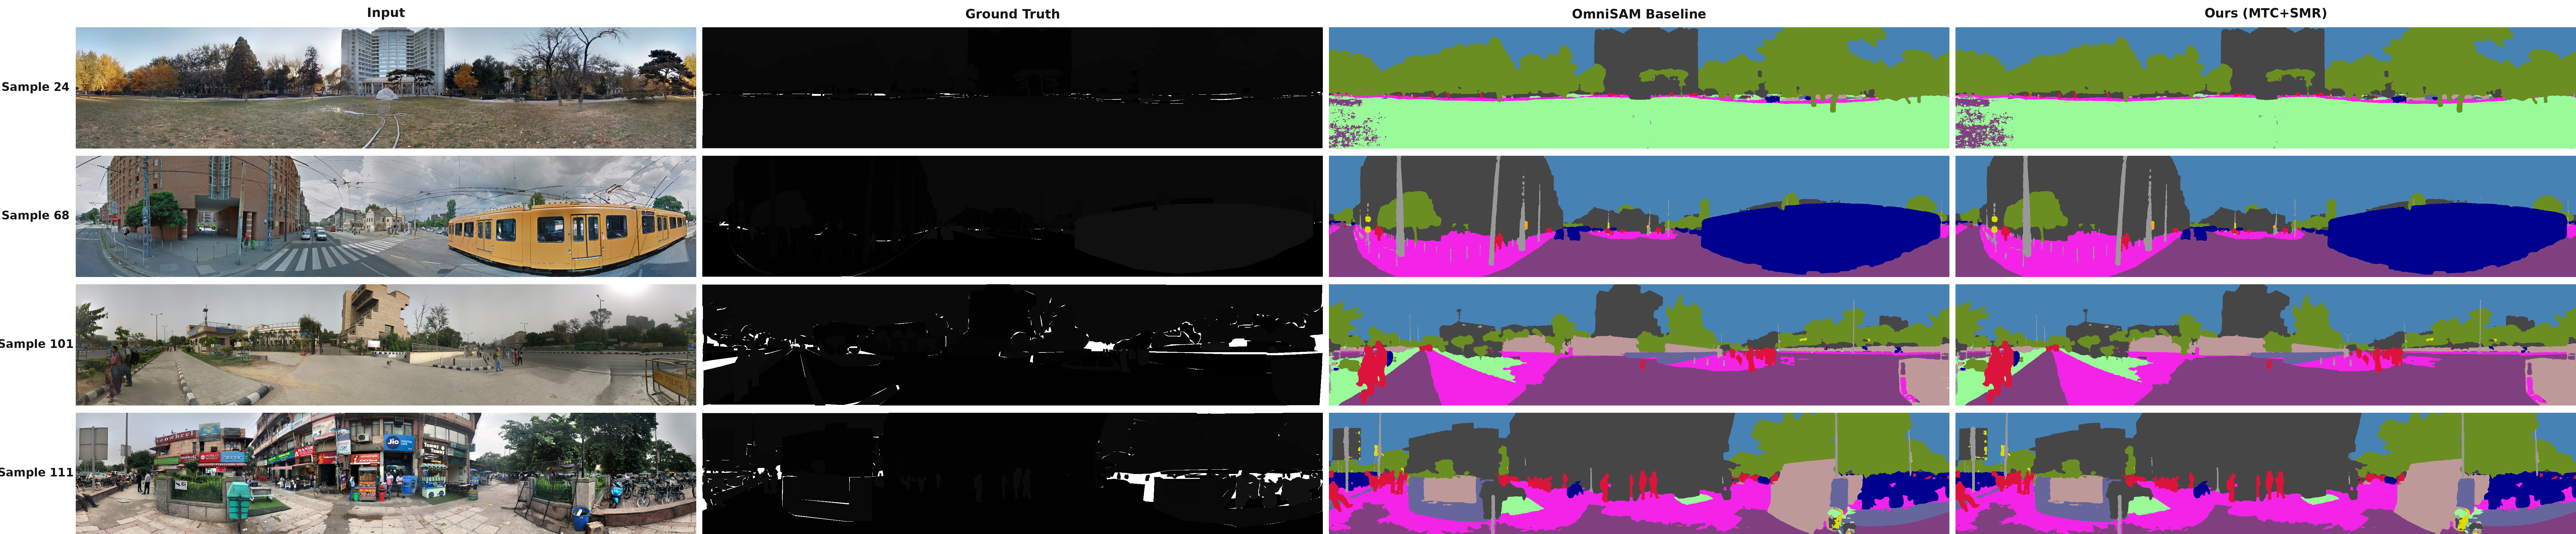
\includegraphics[width=\linewidth]{figures/fig_qualitative_full_protocol.png}
    \caption{Qualitative segmentation results under Cityscapes $\rightarrow$ DensePASS full protocol. Each row shows target domain input, ground truth, OmniSAM baseline prediction, and our MTC+SMR configuration prediction. Baseline and Ours use the same sam2\_s, 13-class protocol, data preprocessing, and ERP inference pipeline.}
    \label{fig:qualitative_full_protocol}
\end{figure}

\section{Ablation Study}
\label{sec:ablation}

\subsection{Memory Module Ablation}
\begin{table}[t]
  \centering
  \small
  \setlength{\tabcolsep}{4pt}
  \renewcommand{\arraystretch}{1.08}
  \caption{Memory-efficient module comparison under fixed pseudo-label ablation setting. This experiment analyzes Memory Tokens and Memory Attention Time, not as full protocol main results.}
  \label{tab:memory_ablation}
  \begin{tabular}{lrrrr}
    \toprule
    Method & Memory Tokens$\downarrow$ & mIoU$\uparrow$ & BFScore$\uparrow$ & Mem. Attn. (s)$\downarrow$ \\
    \midrule
    OmniSAM & 32768 & 60.26 & 39.59 & 117.48 \\
    OmniSAM + Confidence Mask & 32768 & 60.26 & 39.59 & 117.56 \\
    OmniSAM + Confidence Mask + MTC & 8192 & 60.12 & 39.23 & 61.00 \\
    OmniSAM + Confidence Mask + SMR & 16384 & 60.09 & 39.23 & 79.69 \\
    OmniSAM + MTC+SMR & 4096 & 60.02 & 39.23 & 52.38 \\
    OmniSAM + Confidence Mask + MTC+SMR & 4096 & 60.02 & 39.23 & 51.92 \\
    \bottomrule
  \end{tabular}
\end{table}


Table~\ref{tab:memory_ablation} adopts a fixed pseudo-label ablation setting, reusing the same pseudo-labels to isolate memory module effects, not replacing the end-to-end main results in Section~\ref{sec:experiments}. OmniSAM + Confidence Mask does not reduce Memory Tokens, and its Memory Attention Time is essentially consistent with OmniSAM, indicating that only changing pseudo-label filtering without reducing attention input cannot obtain computational gains from this module. After separately enabling MTC or SMR on top of Confidence Mask, Memory Tokens and Memory Attention Time decrease synchronously, verifying that both spatial aggregation and content selection can reduce historical memory interaction. The combined configuration further compresses tokens from 32768 to 4096 and reduces attention time to 51.92s, while accompanied by slight mIoU and BFScore costs, reflecting efficiency-accuracy trade-offs.

As shown in Figure~\ref{fig:speed_accuracy_tradeoff}, memory-efficient configurations trade small accuracy changes for training efficiency gains. The points of different modules do not form a monotonic accuracy improvement relationship, further indicating that the main value of MTC and SMR is controlling training cost rather than enhancing segmentation accuracy. This figure is used for module trend analysis and is not part of full protocol main results.

\begin{figure}[t]
    \centering
    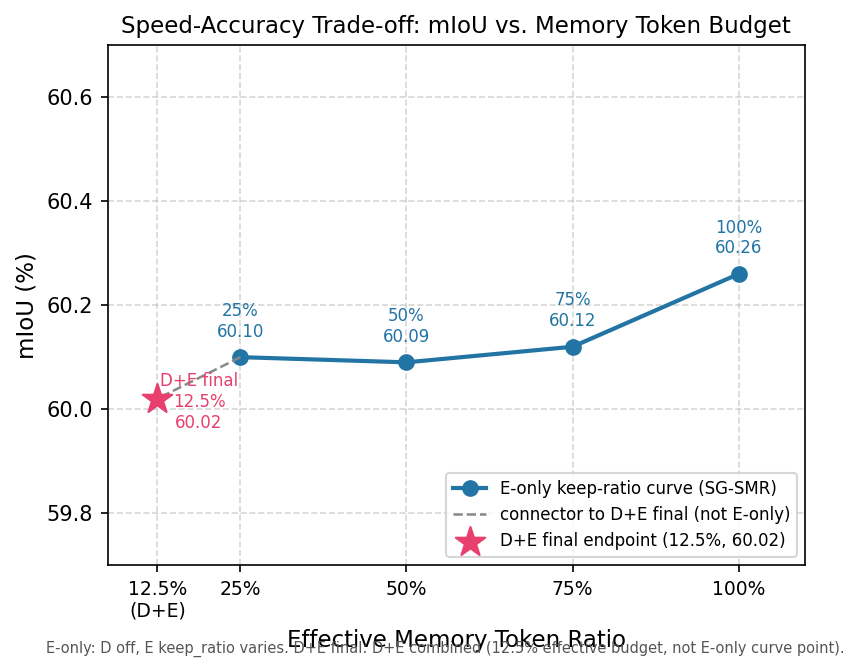
\includegraphics[width=0.78\linewidth]{figures/fig_speed_accuracy_tradeoff_miou.png}
    \caption{Training efficiency vs. mIoU trade-off under fixed pseudo-label ablation setting. Different configurations demonstrate efficiency gains from memory token reduction and corresponding accuracy changes. This figure is not part of full protocol main results.}
    \label{fig:speed_accuracy_tradeoff}
\end{figure}

\subsection{Token Budget}
\begin{table}[t]
  \centering
  \small
  \setlength{\tabcolsep}{3pt}
  \renewcommand{\arraystretch}{1.08}
  \caption{Accuracy and efficiency trade-offs under different Memory Token budgets. Results from fixed pseudo-label ablation setting.}
  \label{tab:token_budget}
  \begin{tabular}{lrrrrr}
    \toprule
    Token Budget & Tokens$\downarrow$ & mIoU$\uparrow$ & BFScore$\uparrow$ & Step (s)$\downarrow$ & Mem. Attn. (s)$\downarrow$ \\
    \midrule
    100\% & 32768 & 60.26 & 39.59 & 2.4089 & 117.56 \\
    75\% & 24576 & 60.12 & 39.28 & 2.4614 & 98.62 \\
    50\% & 16384 & 60.09 & 39.23 & 2.3798 & 79.69 \\
    25\% & 8192 & 60.10 & 39.29 & 2.2941 & 60.54 \\
    12.5\%$^{\dagger}$ & 4096 & 60.02 & 39.23 & 2.3153 & 51.92 \\
    \bottomrule
  \end{tabular}

  \vspace{0.3em}
  \footnotesize{$^{\dagger}$100\%--25\% is the Token Budget curve using only sparse retrieval; 12.5\% is the MTC+SMR combination endpoint.}
\end{table}


Table~\ref{tab:token_budget} and Figure~\ref{fig:token_budget_attention} show that Memory Attention Time generally decreases as Token Budget decreases, while mIoU and BFScore only fluctuate within a small range. This trend directly links computational changes to effective memory token count, also indicating that some historical context can be reduced without causing overall prediction collapse. 100\%--25\% constitutes a Token Budget curve using only SMR, for comparing retention ratios of the same sparse retrieval mechanism; 12.5\% / 4096 tokens is the MTC+SMR combination endpoint and cannot be viewed as a natural extension of this curve. Step Time is not strictly monotonic, indicating that costs such as top-k selection, encoding/decoding, and data processing jointly affect single-step time; Memory Attention Time is more suitable for explaining the direct effect of Token Budget.

\begin{figure}[t]
    \centering
    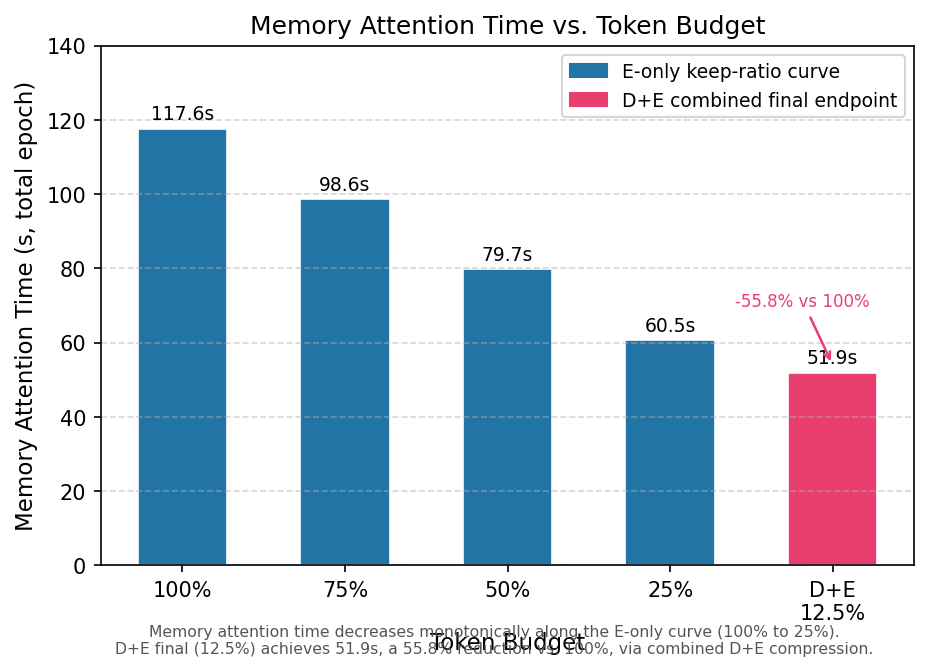
\includegraphics[width=0.78\linewidth]{figures/fig_token_budget_attention_time.png}
    \caption{Relationship between Token Budget and Memory Attention Time under fixed pseudo-label ablation setting. 100\%--25\% is the curve using only SMR, with 12.5\% being the MTC+SMR combination endpoint.}
    \label{fig:token_budget_attention}
\end{figure}

\subsection{Auxiliary PQR Ablation}
\begin{table}[t]
  \centering
  \small
  \setlength{\tabcolsep}{4pt}
  \renewcommand{\arraystretch}{1.08}
  \caption{Auxiliary pseudo-label quality ablation under fixed pseudo-label setting. Results only used to explore supervision reliability, not constituting main performance conclusions of this paper.}
  \label{tab:pseudo_label_ablation}
  \begin{tabular}{lccc}
    \toprule
    Method & mIoU$\uparrow$ & vs. R0 & vs. Previous \\
    \midrule
    Identity (R0) & 60.02 & -- & -- \\
    Class-balanced Filtering (R2) & 60.07 & +0.05 & +0.05 \\
    + Prototype-guided Gating (R2+R4) & 60.05 & +0.03 & -0.02 \\
    \bottomrule
  \end{tabular}
\end{table}


In Table~\ref{tab:pseudo_label_ablation}, mIoU for Identity, class-balanced filtering, and prototype-guided gating are 60.02, 60.07, and 60.05, respectively. Class-balanced filtering only brings $+0.05$, indicating that adjusting class coverage may slightly improve target domain supervision, but the change magnitude is insufficient to support strong conclusions; adding prototype gating does not further improve. One possible reason is that additional filtering reduces effective supervision, or batch-level prototypes remain unstable for rare classes and domain shift. Since these interpretations have not yet been verified by more diagnostics, PQR serves only as auxiliary exploration of pseudo-label reliability and does not constitute the main contribution.

Synthesizing ablation results, MTC+SMR has the most direct evidence for reducing memory attention overhead, but lower token budgets increase risks of fine-grained semantic and boundary losses. Module ablation explains the source of efficiency gains, token budget defines compression strength, and PQR only supplements supervision reliability analysis; the experimental roles of the three cannot be exchanged. Training efficiency and segmentation quality need to be jointly balanced.

\section{Discussion}
\label{sec:discussion}

\subsection{Limitations}
The current experiments are limited to single random seed and single target dataset (DensePASS). Multi-seed validation and cross-dataset generalization (e.g., WildPASS) remain to be verified. The efficiency gains are demonstrated only for training phase; inference acceleration and memory reduction have not been validated. The proposed MTC+SMR may have different effects under different backbone architectures or memory bank configurations.

\subsection{Boundary and Small Object Analysis}
The slight BFScore degradation indicates that token compression affects boundary quality. Further per-class analysis on boundary-sensitive classes (poles, traffic signs) and spatial distribution analysis could provide deeper insights into where the compression impacts prediction quality.

\subsection{Future Directions}
Future work will include: 1) Multi-seed statistical validation to confirm stability; 2) Cross-dataset evaluation on WildPASS and other panoramic datasets; 3) Inference-time efficiency analysis including latency and memory footprint; 4) Investigation of adaptive token budget strategies that adjust compression rates based on scene complexity; 5) Extension to other memory-based architectures beyond OmniSAM.

\section{Conclusion}
\label{sec:conclusion}

This paper addresses memory token redundancy in OmniSAM panoramic UDA training by proposing MTC and SMR: the former restores spatial structure of memories and aggregates adjacent redundancy, while the latter sparsely selects historical tokens based on importance. Their cascade reduces the input scale to memory attention while keeping the visual backbone, segmentation task, and training loss definitions unchanged, thereby confining optimization focus to the memory computation path during training.

In Cityscapes $\rightarrow$ DensePASS experiments with sam2\_s on 13 classes using a single seed, mIoU changes from 60.26 to 60.16 and BFScore from 39.97 to 39.86; total training time decreases from 43m53s to 34m03s, with single iteration time dropping from 5.2655s to 4.0848s, representing approximately 22.4\% time reduction. Results indicate that this method trades slight segmentation quality for clear training efficiency gains. Module ablation and token budget analysis further link these gains to memory token count and attention overhead, while qualitative results show that major scene structures do not experience overall collapse.

Current evidence remains limited to a single target dataset and random seed, and cannot yet support conclusions about cross-dataset stability, inference acceleration, or memory savings; PQR also only provides auxiliary exploration. Future work will supplement multi-seed validation, additional panoramic datasets, and boundary and small object analysis, as well as investigate more reliable cross-field supervision signals.


% Acknowledgments (optional)
\section*{Acknowledgments}
This work was supported by [Funding Agency]. We thank the reviewers for their valuable feedback.

% References
\bibliographystyle{IEEEtran}
\bibliography{refs}

\end{document}
